% =============================================================
% IEEE iSPEC 2026 Conference Paper  -- VERSION 2
% Title: A Two-Stage Deep Learning Pipeline for Automated
%        Cell-Level Extraction and Defect Triage in
%        Photovoltaic Modules
% Template: IEEE Conference Template (062824)
% Rules: IEEEtran, two-column, max 6 pages
% =============================================================

\documentclass[conference]{IEEEtran}
\IEEEoverridecommandlockouts

\usepackage{cite}
\usepackage{amsmath,amssymb,amsfonts}
\usepackage{algorithmic}
\usepackage{graphicx}
\usepackage{textcomp}
\usepackage{xcolor}
\usepackage{booktabs}
\usepackage{multirow}
\usepackage{url}

\def\BibTeX{{\rm B\kern-.05em{\sc i\kern-.025em b}\kern-.08em
    T\kern-.1667em\lower.7ex\hbox{E}\kern-.125emX}}

\begin{document}

% ================================================================
%  TITLE
% ================================================================
\title{A Two-Stage Deep Learning Pipeline for Automated\\
Cell-Level Extraction and Defect Triage in\\
Photovoltaic Modules%
\thanks{This work was carried out at the Indian Institute of
Technology Mandi. The authors gratefully acknowledge the
support of IIT Mandi and the guidance of their research
supervisor.}
}

% ================================================================
%  AUTHORS
% ================================================================
\author{%
\IEEEauthorblockN{1\textsuperscript{st} \textbf{[Author 1 Name]}}
\IEEEauthorblockA{\textit{\textbf{[Department]}} \\
\textit{Indian Institute of Technology Mandi}\\
Mandi, Himachal Pradesh, India \\
\textbf{[email@iitmandi.ac.in]}}
\and
\IEEEauthorblockN{2\textsuperscript{nd} \textbf{[Author 2 Name]}}
\IEEEauthorblockA{\textit{\textbf{[Department]}} \\
\textit{Indian Institute of Technology Mandi}\\
Mandi, Himachal Pradesh, India \\
\textbf{[email@iitmandi.ac.in]}}
}

\maketitle

% ================================================================
%  ABSTRACT
% ================================================================
\begin{abstract}
Automated visual inspection of photovoltaic (PV) modules is
essential for scalable quality control, yet existing approaches
assume pre-cropped, single-cell inputs and reduce defect
assessment to coarse binary labels.
This paper presents a two-stage deep learning pipeline that
operates directly on raw module-level electroluminescence (EL)
images---full and partial captures spanning monocrystalline and
polycrystalline technologies.
Stage~1 performs cell extraction using YOLOv8-OBB (oriented
bounding boxes), adopted after a systematic evaluation of
fifteen classical OpenCV-based approaches across two dataset
tracks (CellExtractOpenCV and FullModuleOpenCV),
none of which generalised robustly.
The YOLOv8-OBB detector, trained on 2{,}212 module images
(80/20 split), outputs five parameters per cell---$(c_x, c_y, w,
h, \theta)$---enabling perspective-correct extraction of
arbitrarily oriented cells without pre-rectification.
Stage~2 performs binary quality triage (OK vs.\ B-grade)
using CNN backbones (ResNet, EfficientNet) augmented with a
Convolutional Block Attention Module (CBAM) and
hyperparameters optimised via Optuna, targeting validation
AUROC under realistic class imbalance.
A third pixel-level defect segmentation stage is identified
as key future work.
We report \textbf{[TBD]} mAP@0.5 for Stage~1 and
\textbf{[TBD]} AUROC for Stage~2.
\end{abstract}

\begin{IEEEkeywords}
photovoltaic inspection, electroluminescence imaging,
YOLOv8-OBB, oriented bounding boxes, binary defect
classification, CBAM, attention mechanism, Optuna,
deep learning, solar energy quality control
\end{IEEEkeywords}

% ================================================================
%  SECTION I --- INTRODUCTION
% ================================================================
\section{Introduction}

Global PV capacity is projected to exceed 10~TW by~2030,
placing unprecedented demands on automated quality assurance
at scale~\cite{iea2023}. Electroluminescence (EL) imaging
detects sub-surface cell defects invisible to conventional
optical inspection, but manual EL review is labour-intensive
and fails to match modern manufacturing throughput or
drone-based fleet inspection rates.

Two critical gaps motivate this work.
\textit{First}, almost every published EL defect study---
including the canonical ELPV benchmark~\cite{deitsch2019}---
assumes individual cell crops as input. In real deployment,
module-level images arrive with arbitrary orientation, partial
occlusion, and perspective distortion; no robust plug-in
extraction stage exists.
\textit{Second}, binary pass/fail classification is the prevailing
paradigm, discarding fault-mechanism information needed for
rework prioritisation and predictive maintenance.

This paper's contributions are:
\begin{enumerate}
  \item A systematic ablation of \textbf{fifteen classical
        OpenCV iterations} (11 on partial/single-cell images,
        4 on full-module images) establishing root-cause
        failure modes of grid-line detection at deployment scale.
  \item A \textbf{YOLOv8-OBB detector} trained on 2{,}212
        module EL images providing unified, format-agnostic
        cell extraction for full-module, partial-module, and
        single-cell inputs.
  \item A \textbf{CBAM-augmented, Optuna-tuned binary triage
        classifier} benchmarked across ResNet-18/50 and
        EfficientNet-B0/B3 backbones on the ELPV dataset
        supplemented with pipeline-extracted crops.
\end{enumerate}

% ================================================================
%  SECTION II --- RELATED WORK
% ================================================================
\section{Related Work}

\subsection{Datasets and Benchmarks}
The ELPV dataset~\cite{deitsch2019} (2{,}624 grayscale cell
crops, 300$\times$300~px) is the canonical EL defect
classification benchmark, but its pre-cropped format leaves
the module-to-cell extraction problem unaddressed.
Full-module industrial EL corpora used in this work span
144-cell (6-string) and 208-cell (8-string) module formats
from multiple manufacturers (ARTS, SDLE, BMRK subsets).

\subsection{Classical Cell Extraction}
Projection profiling~\cite{wong1982}, Hough-transform line
detection~\cite{duda1972}, morphological grid
extraction~\cite{soille2003}, and DBSCAN line clustering are
standard approaches. Their shared weakness is reliance on
image-specific hyperparameters that do not transfer across
module formats, EL contrast levels, or camera orientations.

\subsection{Deep Learning Detection}
YOLO-family detectors~\cite{redmon2016,jocher2023} achieve
state-of-the-art speed-accuracy trade-offs in industrial
inspection. YOLOv8-OBB extends axis-aligned detection with
a learned rotation angle~$\theta$, enabling direct extraction
of arbitrarily oriented PV cells without pre-rectification.

\subsection{Defect Classification}
ResNet~\cite{he2016} and EfficientNet~\cite{tan2019} dominate
EL defect classification. CBAM~\cite{woo2018} appends
channel-wise and spatial-wise attention to any CNN backbone;
Optuna~\cite{akiba2019} provides efficient Bayesian
hyperparameter search superior to grid or random strategies.

% ================================================================
%  SECTION III --- DATASET
% ================================================================
\section{Dataset}

\subsection{Stage 1 --- Module-Level EL Images}

The Stage~1 dataset comprises high-resolution JPEG EL
captures of commercial PV modules acquired under controlled
imaging conditions.
\begin{itemize}
  \item \textbf{Module formats:} 144-cell (12$\times$12,
        6-string) and 208-cell (8$\times$26, 8-string).
  \item \textbf{Size:} 2{,}212 full-module images.
  \item \textbf{Split:} 1{,}769 train / 443 val (80/20),
        partitioned at module level to prevent cell-level
        data leakage.
  \item \textbf{Classical subsets:} ARTS, SDLE, and BMRK
        subsets were used during the 15-notebook classical
        exploration phase to evaluate cross-dataset generalisation.
\end{itemize}

\subsection{Stage 2 --- Cell-Level Triage Images}

Binary triage training data combines the ELPV
dataset~\cite{deitsch2019} with cell crops extracted by
the Stage~1 pipeline.
Labels are binarised: \textit{OK} (functional) vs.\
\textit{B-grade} (any defect present).
A module-level train/val/test split is applied to prevent
spatial correlations across folds.

\subsection{Preprocessing}
All EL images are loaded as single-channel 8-bit grayscale.
The shared preprocessing chain is:
(i)~median blur (3$\times$3 kernel) to suppress sensor
read-out noise;
(ii)~CLAHE (clipLimit\,=\,2.0, tileGridSize\,=\,8$\times$8)
to normalise non-uniform EL emission;
(iii)~perspective correction via
\texttt{cv2.warpPerspective} to produce canonical upright
cell crops; and
(iv)~standard normalisation (zero-mean, unit-std) before
deep learning inference.

% ================================================================
%  SECTION IV --- METHODOLOGY
% ================================================================
\section{Methodology}

\subsection{Stage 1 --- Cell Extraction}
\label{sec:stage1}

\subsubsection{Phase A: CellExtractOpenCV (pp1--pp11)}

Eleven notebooks systematically explored classical extraction
on partial-module and single-cell images from the ARTS, SDLE,
and BMRK datasets. Table~\ref{tab:classical_cell} summarises
each iteration and its primary failure mode.

\begin{table}[t]
  \caption{CellExtractOpenCV: 11-notebook failure summary}
  \label{tab:classical_cell}
  \begin{center}
  \renewcommand{\arraystretch}{1.05}
  \small
  \begin{tabular}{p{0.8cm}p{2.0cm}p{3.5cm}}
    \toprule
    \textbf{NB} & \textbf{Technique} &
    \textbf{Key Limitation} \\
    \midrule
    pp1  & CLAHE + intensity profiles & Exploratory; no extraction \\
    pp2  & Morph.\ grid + persp.\ warp & Single image; not generalised \\
    pp3  & Inversion + contour & Conflates cell with bright defects \\
    pp4  & Batched \texttt{extract\_middle\_cell()} & \textbf{5--10\,\% skip rate on ARTS} \\
    pp5  & ---                  & YOLO pivot notebook \\
    pp6  & Gaussian + Canny     & Fragmented contours \\
    pp7  & NL-Means + Hough     & Image-specific dist.\ threshold \\
    pp8  & Same on multi-cell   & Requires a~priori line count \\
    pp9  & Otsu + Canny         & Format-specific count limit \\
    pp10 & Otsu + contour poly. & Fails on multi-cell images \\
    pp11 & Hough + DBSCAN       & Dataset-specific $\epsilon$ tuning \\
    \bottomrule
  \end{tabular}
  \end{center}
\end{table}

Four root-cause failure modes were identified across all
eleven iterations:
\begin{enumerate}
  \item \textit{Hyperparameter brittleness}---CLAHE clip
        limits, Hough thresholds, morphological kernel
        sizes, and DBSCAN~$\epsilon$ values tuned for one
        image or subset fail on the next.
  \item \textit{Module format sensitivity}---the
        projection-peak detector counted 9 horizontal lines
        for one module and 8 for the next module of the same
        physical format, yielding 208 vs.\ 182 cells.
  \item \textit{Contrast variability}---EL emission varies
        with cell temperature, degradation state, and busbar
        geometry; low-contrast regions cause grid detectors
        to miss busbar lines below the adaptive threshold.
  \item \textit{Perspective intolerance}---morphological
        horizontal/vertical kernels assume axis-aligned
        structure; even 5--10$^\circ$ of module tilt causes
        systematic misdetection.
\end{enumerate}

\subsubsection{Phase B: FullModuleOpenCV (fmv1--fmv4)}

A separate four-notebook track targeted full-resolution
module images (144--208 cells each). Table~\ref{tab:classical_full}
summarises the progression.

\begin{table}[t]
  \caption{FullModuleOpenCV: 4-notebook progression}
  \label{tab:classical_full}
  \begin{center}
  \renewcommand{\arraystretch}{1.05}
  \small
  \begin{tabular}{p{0.7cm}p{2.2cm}p{3.3cm}}
    \toprule
    \textbf{NB} & \textbf{Technique} &
    \textbf{Outcome / Limitation} \\
    \midrule
    fmv1 & HoughLinesP on 2000\,px-wide module &
           Near-duplicate lines; unusable \\
    fmv2 & autocrop + projection-profile peaks &
           \textbf{144 cells from one module}; format-specific \\
    fmv3 & Batch fmv2 across modules &
           208 vs.\ 182 cells (same format) \\
    fmv4 & DBSCAN line merging on 10 modules &
           Partial success; manual count verification needed \\
    \bottomrule
  \end{tabular}
  \end{center}
\end{table}

Despite fmv4 being the best classical result, it still required
format-specific peak-detection parameters, provided no
perspective correction, and could not handle partial-module
views. These limitations motivated the final pivot.

\subsubsection{Phase C: YOLOv8-OBB (Unified Final Approach)}
\label{sec:yolo}

YOLOv8-OBB (Ultralytics~8.3.235)~\cite{jocher2023} was
adopted as the sole Stage~1 detector. Each detection produces
five parameters:
\begin{equation}
  \mathbf{d} = (c_x,\; c_y,\; w,\; h,\; \theta),
  \label{eq:obb}
\end{equation}
where $\theta$ is the rotation angle relative to horizontal.
This directly addresses all four classical failure modes:
format agnosticism through learned features; rotation
robustness via OBB; scale invariance from the multi-scale
feature pyramid; and unified coverage of full-module,
partial-module, and single-cell inputs with a single model.

The post-processing pipeline converts each detection to a
rectified cell crop:
\begin{equation}
  (c_x, c_y, w, h, \theta)
  \;\xrightarrow{\text{corners}}
  M_{\text{persp}}
  \;\xrightarrow{\texttt{warpPerspective}}
  \hat{I}_{\text{cell}}
  \label{eq:postproc}
\end{equation}
where $\hat{I}_{\text{cell}}$ is the canonical
perspective-corrected crop passed to Stage~2.

Fig.~\ref{fig:yolo_detections} shows representative
YOLOv8-OBB detections on a full-module EL image and the
resulting rectified cell crops.

\begin{figure}[t]
  \centering
  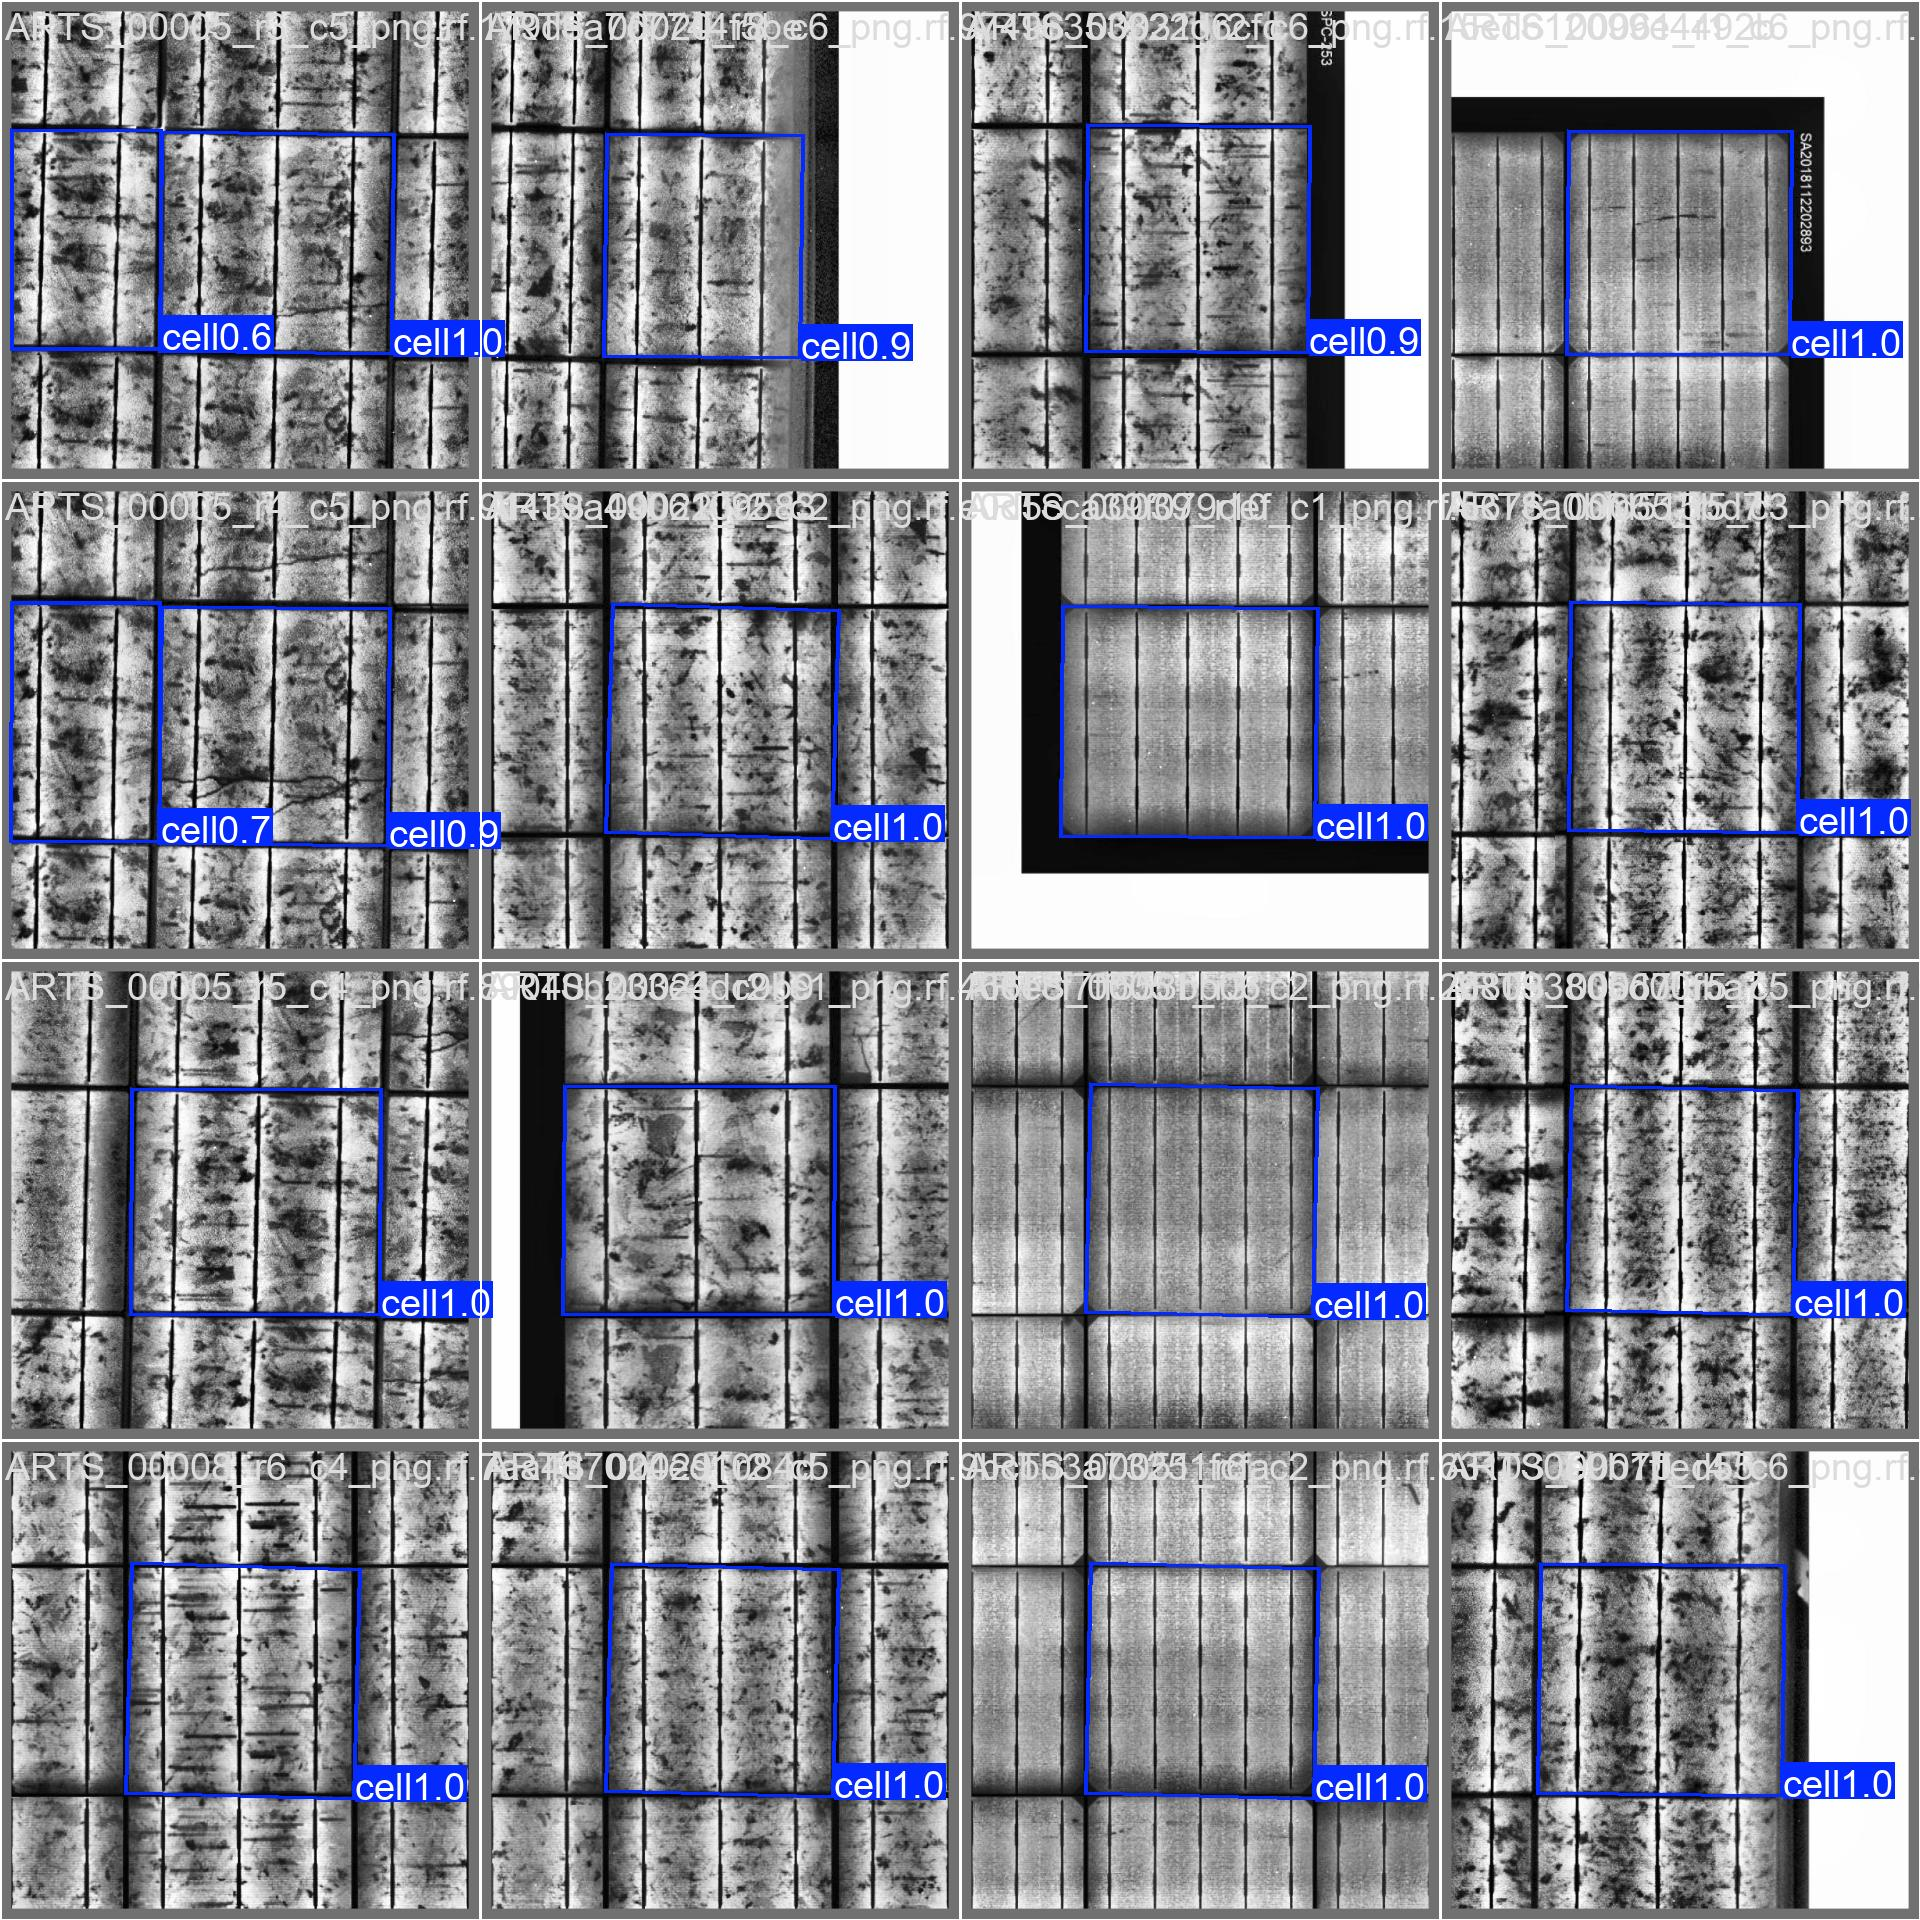
\includegraphics[width=\columnwidth]{fig_yolo_detections.png}
  \caption{YOLOv8-OBB detections on a full-module EL image
           (top) with oriented bounding boxes colour-coded by
           confidence, and resulting perspective-corrected
           cell crops (bottom). Tilted module demonstrates
           OBB rotation robustness.}
  \label{fig:yolo_detections}
\end{figure}

Evaluation metrics include mAP@0.5 and mAP@0.5:0.95
(OBB-adjusted polygon IoU), extraction completeness rate
(detected cells / ground-truth cells per module), and
over-segmentation rate (false-positive detections per module),
reported separately for 144-cell and 208-cell formats.

\subsection{Stage 2 --- Binary Quality Triage}
\label{sec:stage2}

\subsubsection{Architecture}

Each rectified cell crop $\hat{I}_{\text{cell}}$ is
classified as OK or B-grade by a pretrained CNN backbone
augmented with a CBAM block~\cite{woo2018} appended after
the final convolutional stage, followed by global average
pooling, a dropout-regularised fully connected layer, and
a sigmoid output.

CBAM applies dual attention sequentially.
\textit{Channel attention} reweights feature channels to
select defect-relevant maps:
\begin{equation}
  \mathbf{M}_c(\mathbf{F}) = \sigma\!\left(
    W_1\!\left(\text{ReLU}\!\left(W_0\,\text{GAP}(\mathbf{F})\right)\right) +
    W_1\!\left(\text{ReLU}\!\left(W_0\,\text{GMP}(\mathbf{F})\right)\right)
  \right)
  \label{eq:cbam_channel}
\end{equation}
\textit{Spatial attention} then suppresses background pixels:
\begin{equation}
  \mathbf{M}_s(\mathbf{F}') = \sigma\!\left(
    f^{7\times7}\!\!\left(
      \left[\text{AvgPool}(\mathbf{F}');\,\text{MaxPool}(\mathbf{F}')\right]
    \right)\right)
  \label{eq:cbam_spatial}
\end{equation}
where $\sigma$ is the sigmoid function, $W_0$, $W_1$ are MLP
weights with reduction ratio~$r$, $f^{7\times7}$ is a
$7{\times}7$ convolution, and
$\mathbf{F}' = \mathbf{M}_c \otimes \mathbf{F}$.
Defect features in EL images typically occupy $<$5\,\% of
cell area, making CBAM's dual attention particularly
effective without localisation annotations.

\subsubsection{Hyperparameter Optimisation via Optuna}

Table~\ref{tab:optuna} lists the hyperparameter search space.
The optimisation objective is validation AUROC, chosen for
its threshold-invariant behaviour under class imbalance.

\begin{table}[t]
  \caption{Optuna hyperparameter search space (Stage~2)}
  \label{tab:optuna}
  \begin{center}
  \renewcommand{\arraystretch}{1.05}
  \begin{tabular}{ll}
    \toprule
    \textbf{Hyperparameter} & \textbf{Search Space} \\
    \midrule
    Learning rate & LogUniform$[10^{-5},\;10^{-2}]$ \\
    Backbone & \{ResNet-18, ResNet-50, EffNet-B0, EffNet-B3\} \\
    CBAM reduction ratio $r$ & \{4, 8, 16\} \\
    Dropout rate & Uniform$[0.1,\;0.5]$ \\
    Batch size & \{16, 32, 64\} \\
    Optimizer & \{Adam, AdamW, SGD+momentum\} \\
    Objective & Validation AUROC \\
    \bottomrule
  \end{tabular}
  \end{center}
\end{table}

\subsubsection{Evaluation}

Metrics are reported as Accuracy, Precision, Recall,
F1-score, and AUROC---computed separately for monocrystalline
and polycrystalline cells. A baseline ablation isolates the
CBAM contribution (rows~1--2 of Table~\ref{tab:stage2_results}:
same backbone, same LR, CBAM toggled) from the Optuna
tuning contribution (rows~3--5).

% ================================================================
%  SECTION V --- EXPERIMENTAL SETUP
% ================================================================
\section{Experimental Setup}

\textbf{Hardware:} \textbf{[TBD: GPU model, VRAM]}.

\textbf{Software stack:} Python~3.x, PyTorch~\textbf{[TBD]},
Ultralytics~8.3.235 (YOLOv8-OBB), \texttt{timm}~\textbf{[TBD]}
(backbone weights), Optuna~\textbf{[TBD]},
OpenCV~4.12.0.88, NumPy~1.26.4, scikit-learn~\textbf{[TBD]},
Matplotlib~3.8.4.

Table~\ref{tab:training_config} summarises the per-stage
training configuration.

\begin{table}[t]
  \caption{Training configuration per stage}
  \label{tab:training_config}
  \begin{center}
  \renewcommand{\arraystretch}{1.05}
  \small
  \begin{tabular}{lll}
    \toprule
    \textbf{Parameter} &
    \textbf{Stage 1 (YOLO-OBB)} &
    \textbf{Stage 2 (CNN)} \\
    \midrule
    Framework    & Ultralytics     & PyTorch + timm \\
    Input res.   & \textbf{[TBD]}  & \textbf{[TBD]} \\
    Epochs       & \textbf{[TBD]}  & Optuna-selected \\
    Batch size   & \textbf{[TBD]}  & Optuna-selected \\
    Optimizer    & \textbf{[TBD]}  & Optuna-selected \\
    LR schedule  & Cosine          & Optuna-selected \\
    Early stop   & patience\,\textbf{[TBD]} & patience\,\textbf{[TBD]} \\
    Random seeds & $\geq 3$        & $\geq 3$ \\
    \bottomrule
  \end{tabular}
  \end{center}
\end{table}

\textbf{Reproducibility:} All experiments use $\geq$3 independent
random seeds. Results are mean$\pm$std across seeds.
Data splits are fixed prior to any training.

% ================================================================
%  SECTION VI --- RESULTS
% ================================================================
\section{Results}

\subsection{Stage 1: Cell Extraction}

Table~\ref{tab:stage1_results} compares YOLOv8-OBB against the
best classical baseline (fmv4) on the validation set.

\begin{table}[t]
  \caption{Stage~1 cell extraction performance}
  \label{tab:stage1_results}
  \begin{center}
  \renewcommand{\arraystretch}{1.05}
  \small
  \begin{tabular}{llcccc}
    \toprule
    \textbf{Model} & \textbf{Format} &
    \textbf{mAP@.5} & \textbf{mAP@.5:.95} &
    \textbf{Compl.} & \textbf{O-Seg} \\
    \midrule
    YOLO-OBB & 144-cell & \textbf{[TBD]} & \textbf{[TBD]} & \textbf{[TBD]} & \textbf{[TBD]} \\
    YOLO-OBB & 208-cell & \textbf{[TBD]} & \textbf{[TBD]} & \textbf{[TBD]} & \textbf{[TBD]} \\
    YOLO-OBB & Partial  & \textbf{[TBD]} & \textbf{[TBD]} & \textbf{[TBD]} & \textbf{[TBD]} \\
    Classical (fmv4) & Full & N/A & N/A & $\sim$90\,\%$^*$ & High \\
    \bottomrule
    \multicolumn{6}{l}{\footnotesize $^*$Estimated; manual verification required.} \\
    \multicolumn{6}{l}{\footnotesize Compl.\,=\,Completeness; O-Seg\,=\,Over-segmentation.}
  \end{tabular}
  \end{center}
\end{table}

\subsection{Stage 2: Binary Quality Triage}

Table~\ref{tab:stage2_results} shows the backbone and CBAM
ablation. CBAM contribution is isolated from Optuna tuning
by comparing rows~1--2 (identical backbone and LR, CBAM
toggled).

\begin{table}[t]
  \caption{Stage~2 binary triage performance}
  \label{tab:stage2_results}
  \begin{center}
  \renewcommand{\arraystretch}{1.05}
  \small
  \begin{tabular}{llcccc}
    \toprule
    \textbf{Backbone} & \textbf{CBAM} &
    \textbf{Optuna} & \textbf{Acc.} &
    \textbf{F1} & \textbf{AUROC} \\
    \midrule
    ResNet-18  & No  & No  & \textbf{[TBD]} & \textbf{[TBD]} & \textbf{[TBD]} \\
    ResNet-18  & Yes & No  & \textbf{[TBD]} & \textbf{[TBD]} & \textbf{[TBD]} \\
    ResNet-50  & Yes & Yes & \textbf{[TBD]} & \textbf{[TBD]} & \textbf{[TBD]} \\
    EffNet-B0  & Yes & Yes & \textbf{[TBD]} & \textbf{[TBD]} & \textbf{[TBD]} \\
    EffNet-B3  & Yes & Yes & \textbf{[TBD]} & \textbf{[TBD]} & \textbf{[TBD]} \\
    \bottomrule
  \end{tabular}
  \end{center}
\end{table}

Results are reported separately for monocrystalline and
polycrystalline cells.

% ================================================================
%  SECTION VII --- DISCUSSION
% ================================================================
\section{Discussion}

\subsection{Why Classical OpenCV Failed at Deployment Scale}

The 15-notebook exploration reveals four root causes.
\textit{Hyperparameter brittleness} manifests at every step:
CLAHE clip limits, Hough thresholds, and DBSCAN~$\epsilon$
values tuned for one image break on the next due to natural
EL emission variation.
\textit{Module format sensitivity} is illustrated by fmv3,
where the projection-peak detector produced 208 cells (9
horizontal lines) for one module and 182 cells (8 horizontal
lines) for another nominally identical module.
\textit{Contrast variability} from field degradation causes
busbar lines in low-EL regions to drop below adaptive
threshold limits, breaking grid isolation.
\textit{Perspective intolerance} of axis-aligned morphological
kernels means that even 5--10$^\circ$ tilt causes systematic
misdetection.
YOLOv8-OBB subsumes all four sensitivities into learned
model weights, at the cost of requiring labelled training data.

\subsection{CBAM for Spatially Localised Defect Features}

EL defects are spatially sparse ($<$5\,\% of cell area)
and spectrally discriminative---dark regions on a brighter
background. CBAM's channel attention selects
defect-relevant feature maps while spatial attention
suppresses the uniform background; together they are
expected to yield measurable F1 and AUROC gains
(Table~\ref{tab:stage2_results}, rows~1 vs.\ 2) without
requiring localisation annotations.

\subsection{Unified vs.\ Split Detector}

An alternative would use separate detectors for full- and
partial-module inputs. The fmv4 experience shows that even
within the full-module track alone, format-specific tuning
is unavoidable classically. A single YOLOv8-OBB model
trained on a mixed corpus generalises across both input
categories, reducing deployment complexity.

\subsection{Limitations}

\begin{itemize}
  \item \textit{Domain gap}: training data are lab EL images;
        field-collected EL introduces compression artefacts,
        variable exposure, and ambient light contamination.
  \item \textit{Severity absent}: the pipeline produces a
        binary label but no continuous severity score,
        limiting maintenance prioritisation.
  \item \textit{Annotation cost}: labelling 2{,}212
        full-module images at the OBB level is labour-intensive;
        larger corpora may require semi-supervised strategies.
\end{itemize}

% ================================================================
%  SECTION VIII --- CONCLUSION AND FUTURE WORK
% ================================================================
\section{Conclusion and Future Work}

We have presented a two-stage automated inspection pipeline
for PV modules operating on raw module-level EL imagery.
A systematic ablation of 15 classical OpenCV approaches
established that grid-line detection cannot robustly
generalise across deployment-scale diversity, motivating
YOLOv8-OBB as a unified Stage~1 cell extractor.
Stage~2 binary triage with CBAM-augmented CNNs and
Optuna-based hyperparameter search addresses the coarse-label
limitation without localisation supervision.

\textbf{Future work} includes:
(1)~\textit{Stage~3 pixel-level defect segmentation} on
B-grade cells, consolidating 29 defect subtypes into four
physically motivated superclasses (crack, inactive area,
corrosion/metallisation, material/surface) and benchmarking
U-Net family against SegFormer~\cite{xie2021} architectures
with combined Dice+Focal loss;
(2)~severity scoring by mapping segmentation outputs to
power-loss metrics from IV-curve characterisation;
(3)~instance-level defect detection (Mask~R-CNN /
YOLOv11-Seg) for defect counting and spatial clustering;
(4)~domain adaptation from lab to field-acquired EL/IR
imagery; and
(5)~embedded GPU benchmarking (NVIDIA Jetson Orin) for
real-time manufacturing-line integration.

% ================================================================
%  ACKNOWLEDGMENT
% ================================================================
\section*{Acknowledgment}

This work was supported by the Indian Institute of Technology
Mandi. The authors thank their research supervisor for
invaluable guidance and support.

% ================================================================
%  REFERENCES
% ================================================================
\bibliographystyle{IEEEtran}
\bibliography{references}

\end{document}
